% Drawing 154/02-6 -- folder 154, batch 02, archive page 26 (PDF page 27).
% Transcription: page de dessins, sans texte : des faisceaux de pseudo-droites orange coupant une droite verte (pleine ou en pointillé), avec leurs arcs noirs, deux marqués $b$ ; un point de concours entouré des étiquettes $b$, $b-1$, $b+1$, $b\pm 2$ \uncertain{lues} en partie à l'envers ; une ellipse verte ; au crayon, deux fuseaux traversés de droites ; une générisation en pointillé vert passant sous deux faisceaux ; enfin un point double traversé d'une flèche orange en pointillé (une spécialisation traversant le sommet)
% Kind: page of drawings: pencils on a line, generisations, spindles. Method 2 (schematic redraw from the facsimile). Status: ok.
% Notes: Whole page of drawings over a printed listing (CRAY2 job banners, 19 Aug 82; not reproduced). The sheet is upside down in the scan: the drawing is now set upright (turned by 180 degrees, coordinates in the turned crop), so that the listing and Grothendieck's labels read the right way up. Groups, as they stand upright: (1) left, four orange lines crossing in two X's between a green line and a dashed green line (one small green arrowhead); (2) bottom centre, an orange line, an X on it and a dashed orange line; (3) bottom left, the green ellipse; (4) bottom right, a green line with four orange lines, two of them meeting in a V above it, black bars between two of them (ending exactly on the lines), labels 4, 4; (4b) three orange lines concurrent at a black point of the green line and a fourth line, with dashed and solid black bars; (4c) below them, an X of orange lines with a dashed green line and a green line (label 5 between the lines); (5) bottom centre, orange arcs and hooks beside a green line, and a star of three orange lines through one computed point, two of them ending in crossbars, a dashed green curve through the point, labels p-1, q, p≥1, q≥3 on one side and p'-1, q', p'≥1, q'≥3 on the other (the transcription has b, b-1, b+1, b±2); (6) middle left, a black spindle (two arcs crossing near their ends) crossed by five lines, labels 4, 3, 4 inside and 4 to the right, and « 3,4,4,4 » written under it; (7) top centre, a dark and a green arc forming a spindle crossed by six orange strokes and an orange stroke along its right end, labels 3, 4, 4, 4, 3 between the strokes; (8) top centre right, two pencil crossings joined by a solid orange arrow (from the lower crossing up to the upper one), a dashed orange line going on upwards from the upper crossing and downwards from the lower one, ending in an arrowhead (the specialisation through the vertex), four short pencil rays round the upper crossing, a big pencil X through the lower one, two short black dashed lines; (9) top right, a green line with a dashed green arc above it, three orange lines through one computed point on the arc and three more on the right (two crossing below the arc), a violet polyline joining the tops of two of them, labels 4, 4 in pencil; (10) right, a black spindle with two pairs of lines crossing on its upper arc and a fifth line; a small spindle with a thick black stretch on its upper arc and two fans of lines from its two ends; a spindle of two crossing arcs cut by four lines, one stretch of a line brown between the arc and a marked point, labels 3, 4, 3, 4, 3; a spindle of a green and a black arc cut by three lines and a pair from a point of the black arc, labels 3, 4, 3, 4, 3. Left out: the printed listing, a faint pencil sign near the top left X. Still differs from the facsimile: groups (8) to (10) and the green spindle (7) were redrawn from the 400 dpi crop for this pass and are to check again; the lines of the black spindle (6) are as in the earlier pass.
% Coordinates: 1 unit = 1 mm = 1/100 of the crop width, in the crop turned by 180 degrees (the sheet is upside down in the scan; bbox in page fractions of the scan: [0.139, 0.073, 0.973, 0.541]).
% Redrawn by Claude (claude-opus-5-5), issue #73, 2026-11-07; not checked by a human; not compiled (no TeX in the session).
% Revised by Claude (claude-opus-5-5) 2026-11-09 (issue #128) after Michel's check: vertices snapped to exact intersections (drawn points on their lines, meeting ends on the stroke they meet, near-concurrent lines through one computed point, curve ends on their rim); labels at \small as in folder 80 batch 3. Status: partial.
% Redrawn by Claude (claude-opus-5-5) 2026-11-09 (issue #128): upper half re-read at 400 dpi, concurrent lines through one computed point, bars ending on their lines, labels \small and rotated 180 degrees as on the page. Status: partial.
% Revised by Claude (claude-opus-5-5) 2026-11-09 after Michel's check (#134): the whole drawing turned upright (180 degrees: the sheet is upside down in the scan), the labels set upright; groups at the top and right (the double point with the dotted arrow, the pencils on the green line, the green spindle with orange strokes, the four spindles) redrawn from the 400 dpi crop; the readable labels added (3,4,4,4 under the black spindle, 3 4 3 4 3 in the spindles, 3 4 4 4 3 in the green spindle, 4 4 above the green line, 5). Not compiled. Status: partial.
% Rights: reproduces part of the work -- behind RENDER_TRANSCRIPTS, never published by itself.
% Revised by Claude (claude-sonnet-5-5) 2026-11-11 after Michel's check (#142): labels read by Michel: p-1, q, p>=4, q>=3 on the right and p'-1, q', p'>=1, q'>=3 on the left; the two labels under the V and the concurrency of the pencil confirmed. Compiled locally. Status: ok.
\documentclass[tikz,border=3pt]{standalone}
\usepackage{amsmath,amssymb}
\usetikzlibrary{patterns,arrows.meta}
\tikzset{Or/.style={orange!90!black}, Ye/.style={yellow!80!orange}, Lg/.style={green!60!black!70}, Dg/.style={green!45!black}, Br/.style={brown!80!black}, Rd/.style={red!85!black}, Bl/.style={blue!70!black}, Gy/.style={black!40}, pencil/.style={black!45}, struck/.style={black!35}, mark/.style={circle,draw,inner sep=1.3pt}, pt/.style={circle,fill,inner sep=0.9pt}, opt/.style={circle,draw,fill=white,inner sep=1.1pt}}
\colorlet{Or}{orange!90!black}\colorlet{Ye}{yellow!80!orange}\colorlet{Lg}{green!60!black!70}\colorlet{Dg}{green!45!black}\colorlet{Br}{brown!80!black}\colorlet{Rd}{red!85!black}\colorlet{Bl}{blue!70!black}\colorlet{Gy}{black!40}
\begin{document}
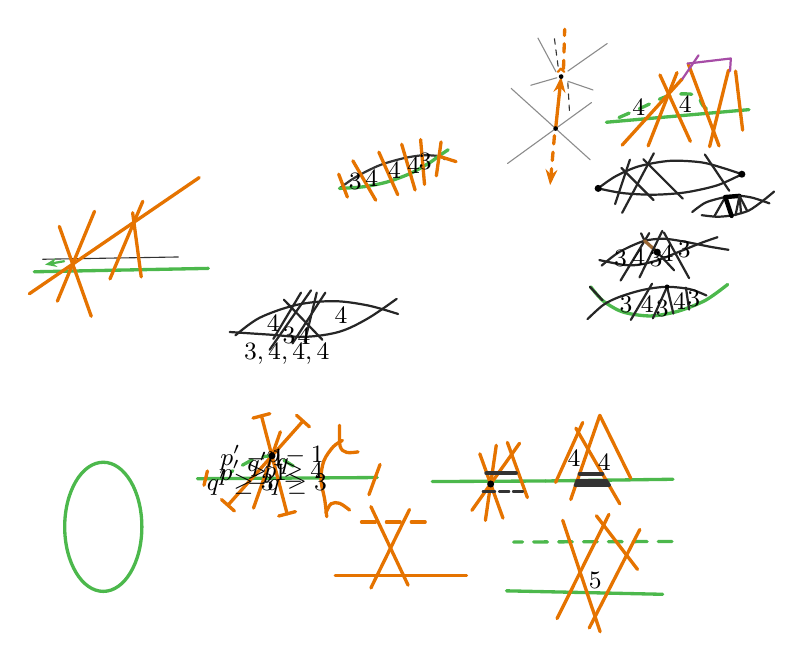
\begin{tikzpicture}[x=1mm,y=1mm,line cap=round,line join=round,font=\scriptsize]
\draw[Lg,very thick] (83.04,-72.75) -- (63.21,-72.31);
\draw[Lg,very thick,dash pattern=on 5pt off 4pt] (84.23,-66.04) -- (64.12,-66.11);
\draw[Or,very thick] (75.1,-77.5) -- (70.35,-63.36);
\draw[Or,very thick] (73.72,-77.02) -- (80.14,-64.52);
\draw[Or,very thick] (69.63,-75.83) -- (76.22,-62.6);
\draw[Or,very thick] (79.85,-69.59) -- (74.63,-62.78);
\draw[Or,very thick] (58.14,-70.32) -- (41.46,-70.32);
\draw[Or,very thick] (50.71,-71.59) -- (45.99,-61.62);
\draw[Or,very thick] (45.99,-71.95) -- (50.89,-61.98);
\draw[Or,very thick,dash pattern=on 5pt off 4pt] (52.88,-63.58) -- (44.18,-63.58);
\draw[Lg,very thick] (12,-64.18) ellipse[x radius=4.9, y radius=8.2];
\draw[Lg,very thick] (84.34,-58.14) -- (68.18,-58.36);
\draw[Or,very thick] (77.6,-61.26) -- (72.02,-51.65);
\draw[Or,very thick] (78.98,-58) -- (75.06,-50.02);
\draw[Or,very thick] (71.37,-60.71) -- (75.06,-50.02);
\draw[Or,very thick] (69.45,-58.54) -- (72.89,-50.93);
\draw[black!80,line width=1.4pt] (76.23,-58.9) -- (71.99,-58.9);
\draw[black!80,line width=1.4pt] (76.08,-58.65) -- (72.08,-58.65);
\draw[black!80,line width=1.4pt] (75.92,-58.36) -- (72.18,-58.36);
\draw[black!80,line width=1.4pt] (75.39,-57.45) -- (72.49,-57.45);
\node[inner sep=1pt] at (75.64,-56) {\small $4$};
\node[inner sep=1pt] at (71.8,-55.46) {\small $4$};
\draw[Lg,very thick] (68.18,-58.36) -- (53.79,-58.43);
\draw[Or,very thick] (62.76,-63.07) -- (59.82,-54.91);
\draw[Or,very thick] (60.53,-63.36) -- (61.91,-53.83);
\draw[Or,very thick] (58.81,-62.09) -- (64.87,-53.57);
\draw[Or,very thick] (65.86,-60.46) -- (63.32,-53.46);
\node[pt] at (61.2,-58.74) {};
\draw[black!80,line width=1.4pt,dash pattern=on 3pt off 2pt] (65.2,-59.7) -- (61.94,-59.7);
\draw[black!80,line width=1.4pt] (61.65,-59.7) -- (60.31,-59.7);
\draw[black!80,line width=1.4pt] (64.41,-57.38) -- (60.64,-57.38);
\draw[Lg,very thick] (46.79,-57.92) -- (23.96,-58.07);
\draw[Or,very thick] (45.74,-60.1) -- (47.15,-56.26);
\draw[Or,very thick] (24.79,-58.9) -- (25.23,-57.09);
\draw[Or,very thick] plot[smooth, tension=0.55] coordinates {(40.38,-62.89) (40.12,-60.71) (39.65,-58.18) (40.01,-55.82) (41.21,-54.01) (42.37,-53.21)};
\draw[Or,very thick] plot[smooth, tension=0.55] coordinates {(43.28,-62.05) (42.01,-61.19) (40.92,-61.26) (40.27,-62.42)};
\draw[Or,very thick] plot[smooth, tension=0.55] coordinates {(44.36,-54.66) (42.91,-54.73) (42.08,-53.94) (42.01,-51.29)};
\draw[Or,very thick] (35.35,-62.53) -- (32.09,-50.09);
\draw[Or,very thick] (31.08,-61.8) -- (34.49,-52.12);
\draw[Or,very thick] (27.83,-61.44) -- (37.36,-50.75);
\draw[Or,very thick] (34.28,-62.81) -- (36.41,-62.25);
\draw[Or,very thick] (31.02,-50.37) -- (33.15,-49.81);
\draw[Or,very thick] (27.01,-60.71) -- (28.65,-62.17);
\draw[Or,very thick] (36.54,-50.01) -- (38.18,-51.48);
\draw[Lg,very thick,dash pattern=on 4pt off 4pt] plot[smooth, tension=0.55] coordinates {(36.14,-56.47) (34.76,-55.64) (33.42,-55.17) (31.13,-55.6) (28.23,-57.2)};
\node[pt] at (33.42,-55.17) {};
\node[inner sep=1pt] at (36.39,-55.28) {\small $p-1$};
\node[inner sep=1pt] at (34.76,-56.47) {\small $q$};
\node[inner sep=1pt] at (36.14,-57.34) {\small $p\geq 4$};
\node[inner sep=1pt] at (36.64,-58.9) {\small $q\geq 3$};
\node[inner sep=1pt] at (30.95,-55.39) {\small $p'-1$};
\node[inner sep=1pt] at (31.57,-56.26) {\small $q'$};
\node[inner sep=1pt] at (31.06,-57.34) {\small $p'\geq 1$};
\node[inner sep=1pt] at (29.39,-58.61) {\small $q'\geq 3$};
\draw[black!85,thick] plot[smooth, tension=0.55] coordinates {(49.26,-35.23) (45.63,-37.7) (42.01,-39.4) (37.66,-40.05) (32.95,-39.76) (28.05,-39.44)};
\draw[black!85,thick] plot[smooth, tension=0.55] coordinates {(49.44,-37.15) (45.63,-36.07) (41.28,-35.52) (36.57,-35.99) (31.86,-37.63) (28.78,-39.87)};
\draw[black!85,thick] (39.83,-40.42) -- (34.94,-35.34);
\draw[black!85,thick] (37.59,-40.67) -- (39.11,-34.44);
\draw[black!85,thick] (36.03,-40.89) -- (40.2,-34.44);
\draw[black!85,thick] (33.6,-40.31) -- (37.11,-34.44);
\draw[black!85,thick] (33.13,-41.69) -- (38.38,-34.15);
\node[inner sep=1pt] at (42.2,-37.3) {\small $4$};
\node[inner sep=1pt] at (37.5,-40) {\small $4$};
\node[inner sep=1pt] at (35.6,-39.9) {\small $3$};
\node[inner sep=1pt] at (33.6,-38.3) {\small $4$};
\draw[Lg,very thick] (25.34,-31.36) -- (3.23,-31.79);
\draw[black!80] (21.53,-29.91) -- (4.31,-30.2);
\draw[Or,very thick] (2.61,-34.58) -- (24.18,-19.83);
\draw[Or,very thick] (10.47,-37.44) -- (6.42,-26.03);
\draw[Or,very thick] (6.17,-35.52) -- (10.89,-24.11);
\draw[Or,very thick] (16.82,-32.44) -- (15.73,-24.29);
\draw[Or,very thick] (12.85,-32.7) -- (17.02,-22.84);
\draw[Lg,thick,-{Stealth[length=1.5mm]}] (7.03,-30.45) -- (4.6,-30.88);
\node[inner sep=1pt] at (35.3,-42.2) {\small $3,4,4,4$};
\node[inner sep=1pt] at (74.5,-71) {\small $5$};
\draw[pencil] (66.3,-8.1) -- (69.6,-7.15);
\draw[pencil] (71,-7.6) -- (74.2,-8.7);
\draw[pencil] (67.2,-2.1) -- (69.5,-6.4);
\draw[pencil] (71,-6.3) -- (76,-2.8);
\draw[pencil] (63.8,-8.5) -- (73.83,-17.56);
\draw[pencil] (74,-10.3) -- (63.35,-18.03);
\draw[Or,very thick,-{Stealth[length=2mm]}] (69.45,-13.6) -- (70.15,-7);
\draw[Or,very thick,dash pattern=on 3pt off 3pt] (70.45,-6) -- (70.6,-1);
\draw[Or,thick] (69.75,-6.4) -- (70.1,-6) -- (70.55,-6.4);
\draw[Or,very thick,dash pattern=on 3pt off 3pt,-{Stealth[length=2mm]}] (69.3,-14.5) -- (68.75,-20.8);
\draw[black!80,dash pattern=on 2pt off 2pt] (69.3,-2.2) -- (69.8,-6);
\draw[black!80,dash pattern=on 2pt off 2pt] (71,-7.8) -- (71.2,-11.3);
\node[pt,pt,inner sep=0.6pt] at (70.15,-7) {};
\node[pt,pt,inner sep=0.6pt] at (69.45,-13.6) {};
\draw[Lg,very thick] (75.9,-12.8) -- (94,-11.2);
\draw[Lg,very thick,dash pattern=on 4pt off 4pt] plot[smooth, tension=0.5] coordinates {(77.5,-12.2) (80.7,-10.8) (83.3,-9.6) (85.4,-9.2) (87.4,-9.4) (88.1,-10.6) (89,-11.45)};
\draw[Or,very thick] (77.9,-15.7) -- (85.51,-7.31);
\draw[Or,very thick] (81.2,-15.8) -- (84.86,-6.5);
\draw[Or,very thick] (82.7,-6.8) -- (86.56,-15.22);
\draw[Or,very thick] (86.3,-5.4) -- (90.2,-15.8);
\draw[Or,very thick] (91.4,-6.2) -- (89,-15.9);
\draw[Or,very thick] (92.3,-6.3) -- (93.2,-13.8);
\draw[violet!70,thick] (85.55,-7.3) -- (87.6,-4.3);
\draw[violet!70,thick] (86.2,-5.35) -- (91.7,-4.7) -- (91.6,-6.3);
\node[inner sep=1pt] at (80,-10.9) {\small $4$};
\node[inner sep=1pt] at (85.9,-10.5) {\small $4$};
\draw[black!80,thick] plot[smooth, tension=0.5] coordinates {(42,-21.2) (44,-19.8) (47,-18.3) (50,-17.4) (52.5,-17) (54.6,-17.1) (55.4,-17.5)};
\draw[Lg,very thick] plot[smooth, tension=0.5] coordinates {(42,-21.2) (45,-21) (48,-20.4) (51,-19.3) (53.5,-17.9) (54.6,-17.1) (55.8,-16.3)};
\draw[Or,very thick] (41.9,-19.4) -- (43,-22.3);
\draw[Or,very thick] (43.7,-17.7) -- (46.6,-22.7);
\draw[Or,very thick] (47,-16.6) -- (49.4,-22);
\draw[Or,very thick] (49.9,-15.6) -- (51.6,-21.4);
\draw[Or,very thick] (52.3,-15) -- (52.8,-20.7);
\draw[Or,very thick] (54.9,-15.3) -- (54.3,-19.6);
\draw[Or,very thick] (54.6,-17.1) -- (56.8,-17.8);
\node[inner sep=1pt] at (44,-20.3) {\small $3$};
\node[inner sep=1pt] at (46.1,-19.95) {\small $4$};
\node[inner sep=1pt] at (49,-18.9) {\small $4$};
\node[inner sep=1pt] at (51.4,-18.3) {\small $4$};
\node[inner sep=1pt] at (52.9,-17.8) {\small $3$};
\draw[black!85,thick] plot[smooth, tension=0.5] coordinates {(74.85,-21.2) (77,-19.7) (80,-18.4) (84,-17.7) (88,-17.9) (91,-18.7) (93.1,-19.4)};
\draw[black!85,thick] plot[smooth, tension=0.5] coordinates {(74.85,-21.2) (78,-21.8) (82,-22) (86,-21.7) (90,-20.8) (93.1,-19.4)};
\draw[black!85,thick] (77,-23.2) -- (78.88,-17.56);
\draw[black!85,thick] (77.8,-18.6) -- (81.89,-22.69);
\draw[black!85,thick] (77.9,-24.3) -- (81.92,-16.74);
\draw[black!85,thick] (80.6,-17.5) -- (85.6,-22.5);
\draw[black!85,thick] (88.4,-16.9) -- (91.5,-21.5);
\node[pt,pt] at (74.85,-21.2) {};
\node[pt,pt] at (93.1,-19.4) {};
\draw[black!85,thick] plot[smooth, tension=0.5] coordinates {(86.8,-24.2) (88.5,-23) (91,-22.3) (92.8,-22.15) (94.5,-22.4) (96.6,-23.1)};
\draw[black,line width=1.6pt] (91,-22.3) -- (92.8,-22.15);
\draw[black!85,thick] plot[smooth, tension=0.5] coordinates {(88,-24.6) (90,-24.8) (92,-24.6) (94,-24) (95.8,-22.75) (97.2,-21.6)};
\draw[black!85,thick] (91,-22.3) -- (89.6,-24.75);
\draw[black,line width=1.6pt] (91,-22.3) -- (91.8,-24.7);
\draw[black!85,thick] (92.8,-22.15) -- (92.3,-24.6);
\draw[black!85,thick] (92.8,-22.15) -- (93,-24.35);
\draw[black!85,thick] (92.8,-22.15) -- (93.8,-24.1);
\draw[black!85,thick] plot[smooth, tension=0.5] coordinates {(75.3,-31) (77.5,-29.3) (80.6,-27.9) (83.2,-27.6) (86,-28) (89,-28.6) (91.4,-29)};
\draw[black!85,thick] plot[smooth, tension=0.5] coordinates {(75,-30.3) (78,-30.9) (80,-30.9) (82.5,-30.3) (85,-29.3) (88,-28.1) (90,-27.4)};
\draw[black!85,thick] (77.7,-32.9) -- (81.34,-26.88);
\draw[black!85,thick] (80.3,-26.9) -- (80.75,-27.85);
\draw[Br,very thick] (80.75,-27.85) -- (82.35,-29.3);
\draw[black!85,thick] (82.35,-29.3) -- (84.5,-31.6);
\draw[black!85,thick] (80.1,-32.5) -- (83,-26.6);
\draw[black!85,thick] (83.2,-26.8) -- (86.4,-32.6);
\node[pt,pt] at (82.35,-29.3) {};
\node[inner sep=1pt] at (77.7,-30.1) {\small $3$};
\node[inner sep=1pt] at (80,-30) {\small $4$};
\node[inner sep=1pt] at (82.2,-30.15) {\small $3$};
\node[inner sep=1pt] at (83.6,-29.5) {\small $4$};
\node[inner sep=1pt] at (85.8,-28.9) {\small $3$};
\draw[Lg,very thick] plot[smooth, tension=0.5] coordinates {(73.9,-33.7) (75.5,-35.5) (78,-36.9) (81.5,-37.4) (85,-36.8) (88.5,-35.4) (91.3,-33.4)};
\draw[black!85,thick] plot[smooth, tension=0.5] coordinates {(73.5,-37.8) (75.5,-36) (77.5,-35) (80.5,-34.1) (83.5,-33.7) (86.5,-34) (88.6,-34.8)};
\draw[black!85,thick] (73.8,-33.7) -- (75.4,-35.4);
\draw[black!85,thick] (79,-37.9) -- (81.7,-33.3);
\draw[black!85,thick] (81.8,-37.7) -- (83.6,-33.7);
\draw[black!85,thick] (83.6,-33.7) -- (84.4,-37.1);
\draw[black!85,thick] (86,-33.8) -- (86.4,-36.6);
\node[pt,pt,inner sep=0.6pt] at (83.6,-33.7) {};
\node[inner sep=1pt] at (78.4,-36) {\small $3$};
\node[inner sep=1pt] at (81.1,-36) {\small $4$};
\node[inner sep=1pt] at (83,-36.5) {\small $3$};
\node[inner sep=1pt] at (85.2,-35.6) {\small $4$};
\node[inner sep=1pt] at (87,-35.2) {\small $3$};
\end{tikzpicture}
\end{document}
